\documentclass[12pt]{article}
%\usepackage[latin1]{inputenc}
\usepackage{pdfsync}
\usepackage{amssymb}
\usepackage{amsmath}
\usepackage{latexsym}
\usepackage{amsthm}
\usepackage{hyperref}
\usepackage{eucal}
\usepackage{indentfirst}
\usepackage{caption}
\usepackage{subcaption}
\usepackage{float}
\usepackage{graphicx} % for figures
\usepackage{amsfonts}
\usepackage{natbib}
\usepackage{sidecap}
\usepackage{setspace}
\usepackage{fancyhdr}
\usepackage{gensymb}
\usepackage{color}
\usepackage{wrapfig}
\usepackage{array}
\usepackage{booktabs}
\usepackage{lastpage}
\usepackage[titletoc]{appendix}
\usepackage{soul}
\usepackage{pythontex}
%\usepackage{ulem}
\usepackage[body={9.0in, 9.0in},left=1 in,right=1in]{geometry} % Geometry package for easy page margin setup\setcounter{MaxMatrixCols}{30}
\linespread{1} % interline
\DeclareGraphicsExtensions{.jpg,.pdf,.mps,.png,.eps}
 

%%%%%%%%%%%%%Colors%%%%%%%%%%%%%%%
\usepackage[dvispnames]{xcolor}
\definecolor{pink}{cmyk}{0, 0.7808, 0.4429, 0.1412}
%%%%%%%%%%%%% Page setup %%%%%%%%%%
\pagestyle{fancy}
\renewcommand{\headrulewidth}{0pt}
%\lhead{\footnotesize \parbox{11cm}{Draft 1} }
\lfoot{\footnotesize Kaushik Dutta \\ Ryan Friedman \\ Siqi Zhao}
%\cfoot{}
%\chead{}
%\rhead{\footnotesize 3}
\rfoot{\footnotesize Page \thepage\ of \pageref{LastPage}}
\newcommand{\noin}{\noindent} 


%%%%%%%%%%%%%%%%%%%%%%%%
%\usepackage{pythonhighlight}
\usepackage{algorithm}
\usepackage[noend]{algpseudocode}
\makeatletter
\def\BState{\State\hskip-\ALG@thistlm}
\makeatother
\usepackage{physics}
%%%%%%%%%%%%%%%%%%%%%%%%%

\begin{document}

\section{Results}
\noin To select the optimal amount of regularization, we tried $\lambda$ values ranging from $10$ to $10^{-5}$ and created an L-curve. Using this criteria, we found that the optimal reconstruction is with $\lambda$ is $2 \times 10^{-4}$ for 540 views, $10^{-3}$ for 270 views, and $2 \times 10^{-4}$ for 90 views (Figure~\ref{fig:lcurves}). The reconstruction from the full sinogram for all values of $\lambda$ is shown in Supplemental Figure~\ref{fig:fullReconstructions}.

% L-curves
\begin{figure}[h]
	\begin{subfigure}[t]{0.3\textwidth}
		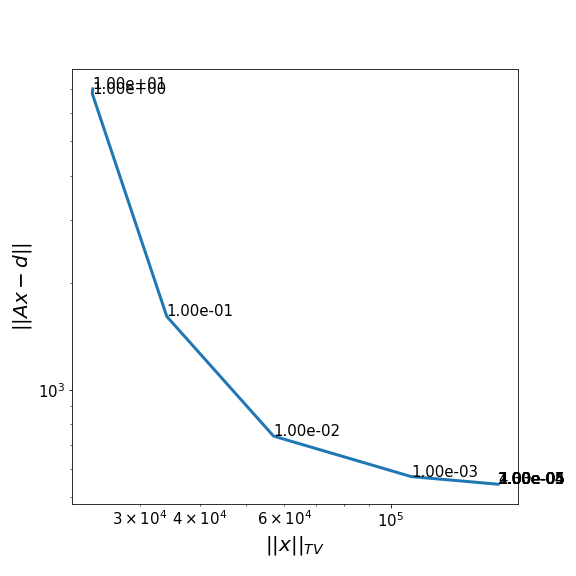
\includegraphics[width=\linewidth]{../results/fistaFullLcurve.png}
		\caption{Full sinogram}
		\label{fig:lcurvefull}
	\end{subfigure}
	\hfill
	\begin{subfigure}[t]{0.3\textwidth}
		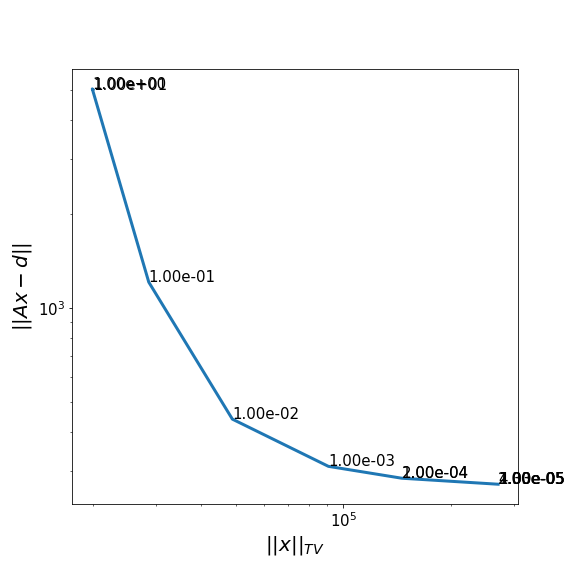
\includegraphics[width=\linewidth]{../results/fista270Lcurve.png}
		\caption{270 views}
		\label{fig:lcurve270}
	\end{subfigure}
	\hfill
	\begin{subfigure}[t]{0.3\textwidth}
		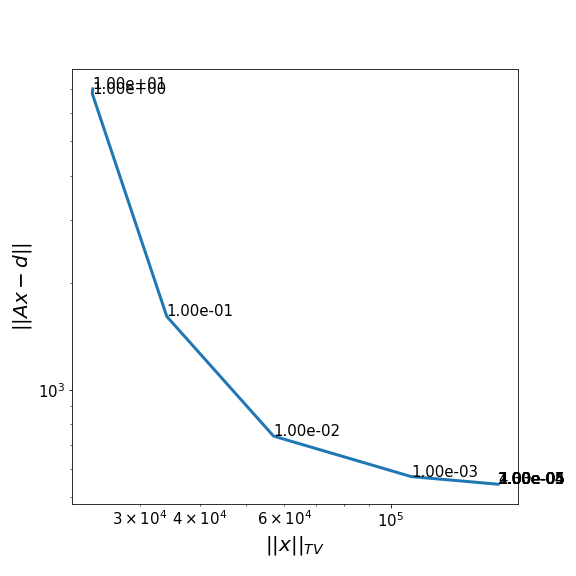
\includegraphics[width=\linewidth]{../results/fistaFullLcurve.png}
		\caption{90 views}
		\label{fig:lcurve90}
	\end{subfigure}
	
	\caption{L-curves for FISTA reconstruction of image.}
	\label{fig:lcurves}
\end{figure}

\noin We compared the image reconstructed with FISTA to reconstructions with SART. We chose to implement SART as our stationary method because it is less prone to overfitting than ART and converges faster than SIRT. We assessed image quality using two metrics, the structural similarity (SSIM) index and the mean squared error (MSE). We computed these metrics on the full image and on a defined region of interest (ROI). We set our ROI to cover pixel rows 175-220 and pixel columns 100-140 because the image has complex shapes in this region. The reconstructed images for 540, 270, and 90 views are shown in Figures~\ref{fig:comparisonfull},~\ref{fig:comparison270}, and~\ref{fig:comparison90}, respectively. The SSIM metrics are shown in Table~\ref{tab:ssim} and the MSE metrics are shown in Table~\ref{tab:mse}. In virtually every case, FISTA outperforms SART. However, SART slightly outperforms FISTA in the following cases:
\begin{itemize}
	\item The SSIM on the full image is higher with SART than with FISTA, although this is not the case for MSE.
	\item The reconstruction of the ROI from 270 views is slightly better with SART than with FISTA.
\end{itemize}

% SSIM metrics
\begin{table}[h]
	\centering
	\begin{tabular}{|c|c|c|c|c|}
		\hline
		\textbf{Number of views} & \textbf{FISTA} & \textbf{FISTA ROI} & \textbf{SART} & \textbf{SART ROI} \\
		\hline
		540 & 0.860 & 0.968 & 0.885 & 0.855 \\
		270 & 0.888 & 0.837 & 0.877 & 0.849 \\
		90  & 0.889 & 0.843 & 0.792 & 0.741 \\
		\hline
	\end{tabular}
	\caption{SSIM of image reconstructions.}
	\label{tab:ssim}
\end{table}

% MSE metrics
\begin{table}[h]
	\centering
	\begin{tabular}{|c|c|c|c|c|}
		\hline
		\textbf{Number of views} & \textbf{FISTA} & \textbf{FISTA ROI} & \textbf{SART} & \textbf{SART ROI} \\
		\hline
		540 & 33.18 &  40.02 & 40.91 & 244.75 \\
		270 & 38.44 & 254.20 & 43.62 & 251.27 \\
		90  & 39.08 & 251.92 & 80.66 & 397.23 \\
		\hline
	\end{tabular}
	\caption{MSE of image reconstructions.}
	\label{tab:mse}
\end{table}

% FISTA and SART side by side: full sinogram
\begin{figure}[H]
	\centering
	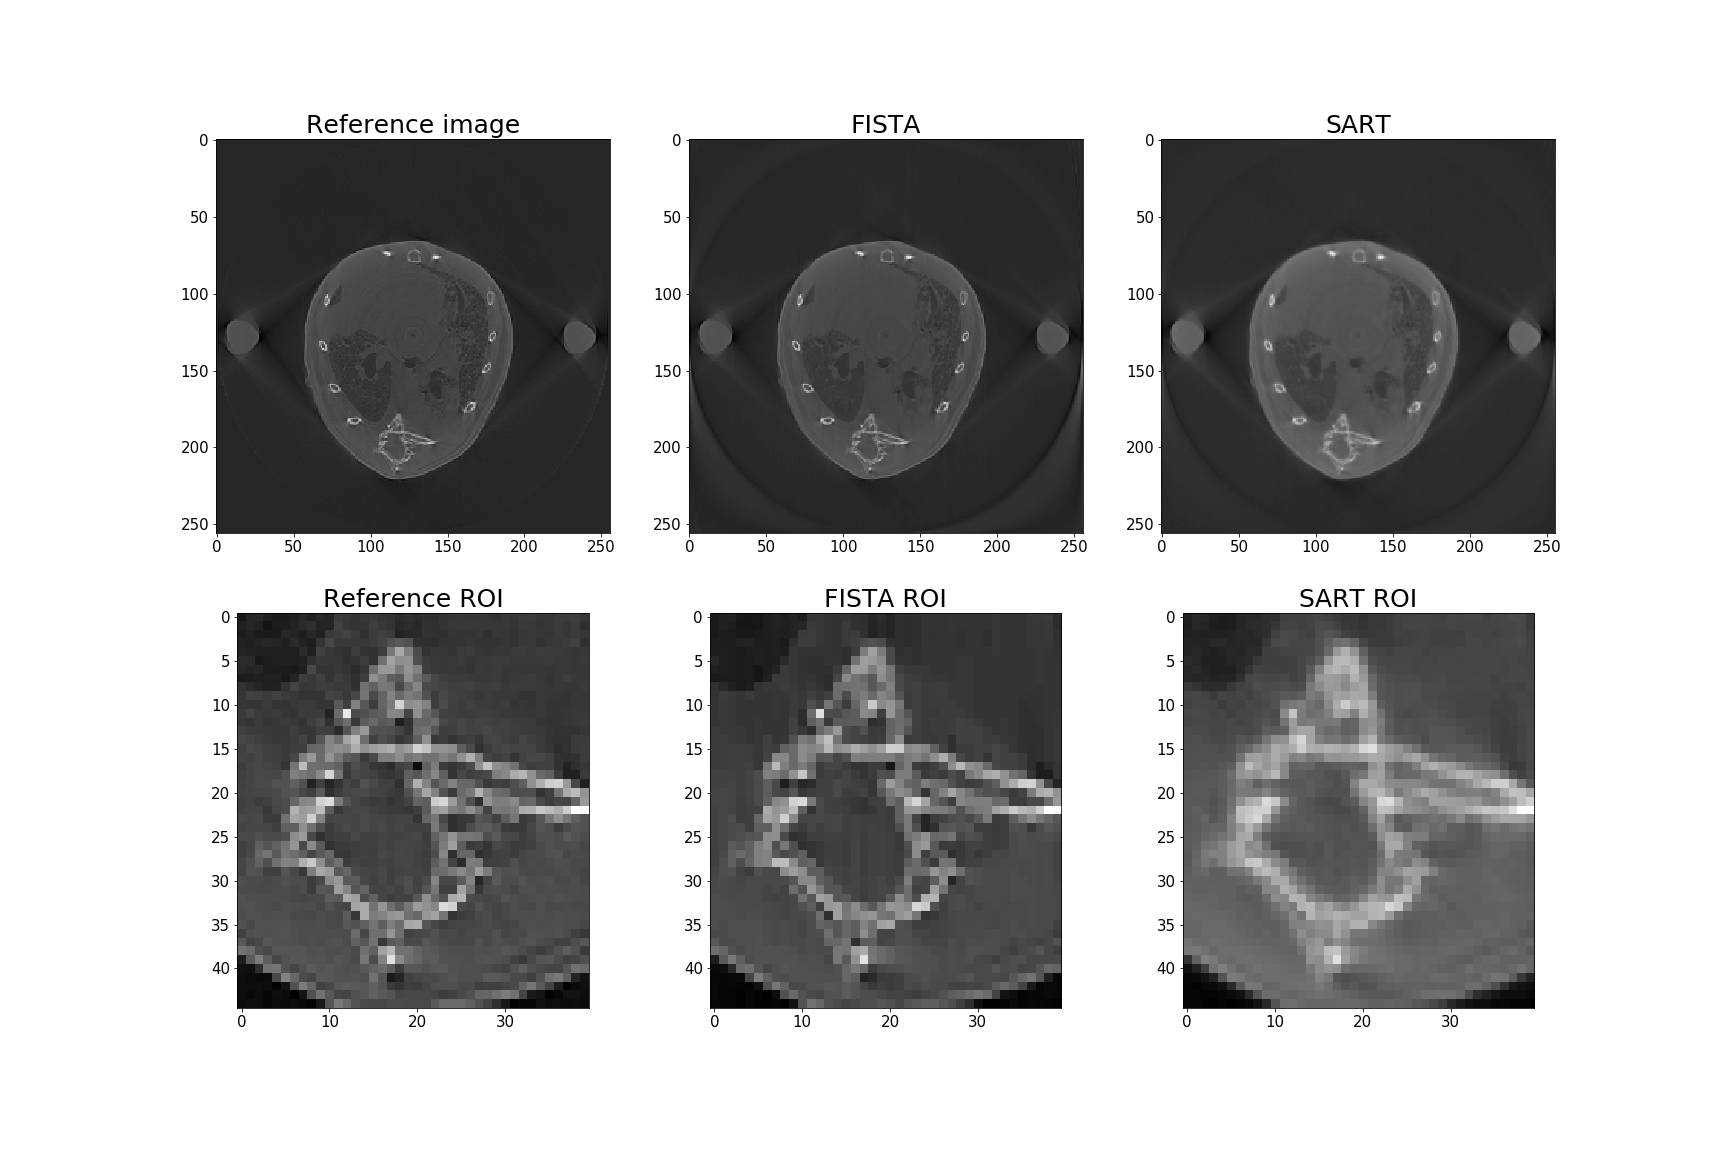
\includegraphics[height=0.35\paperheight]{../results/comparisonFull.png}
	\caption{Reconstructed image using FISTA and SART from the full sinogram.}
	\label{fig:comparisonfull}
\end{figure}

% FISTA and SART side by side: 270
\begin{figure}[H]
	\centering
	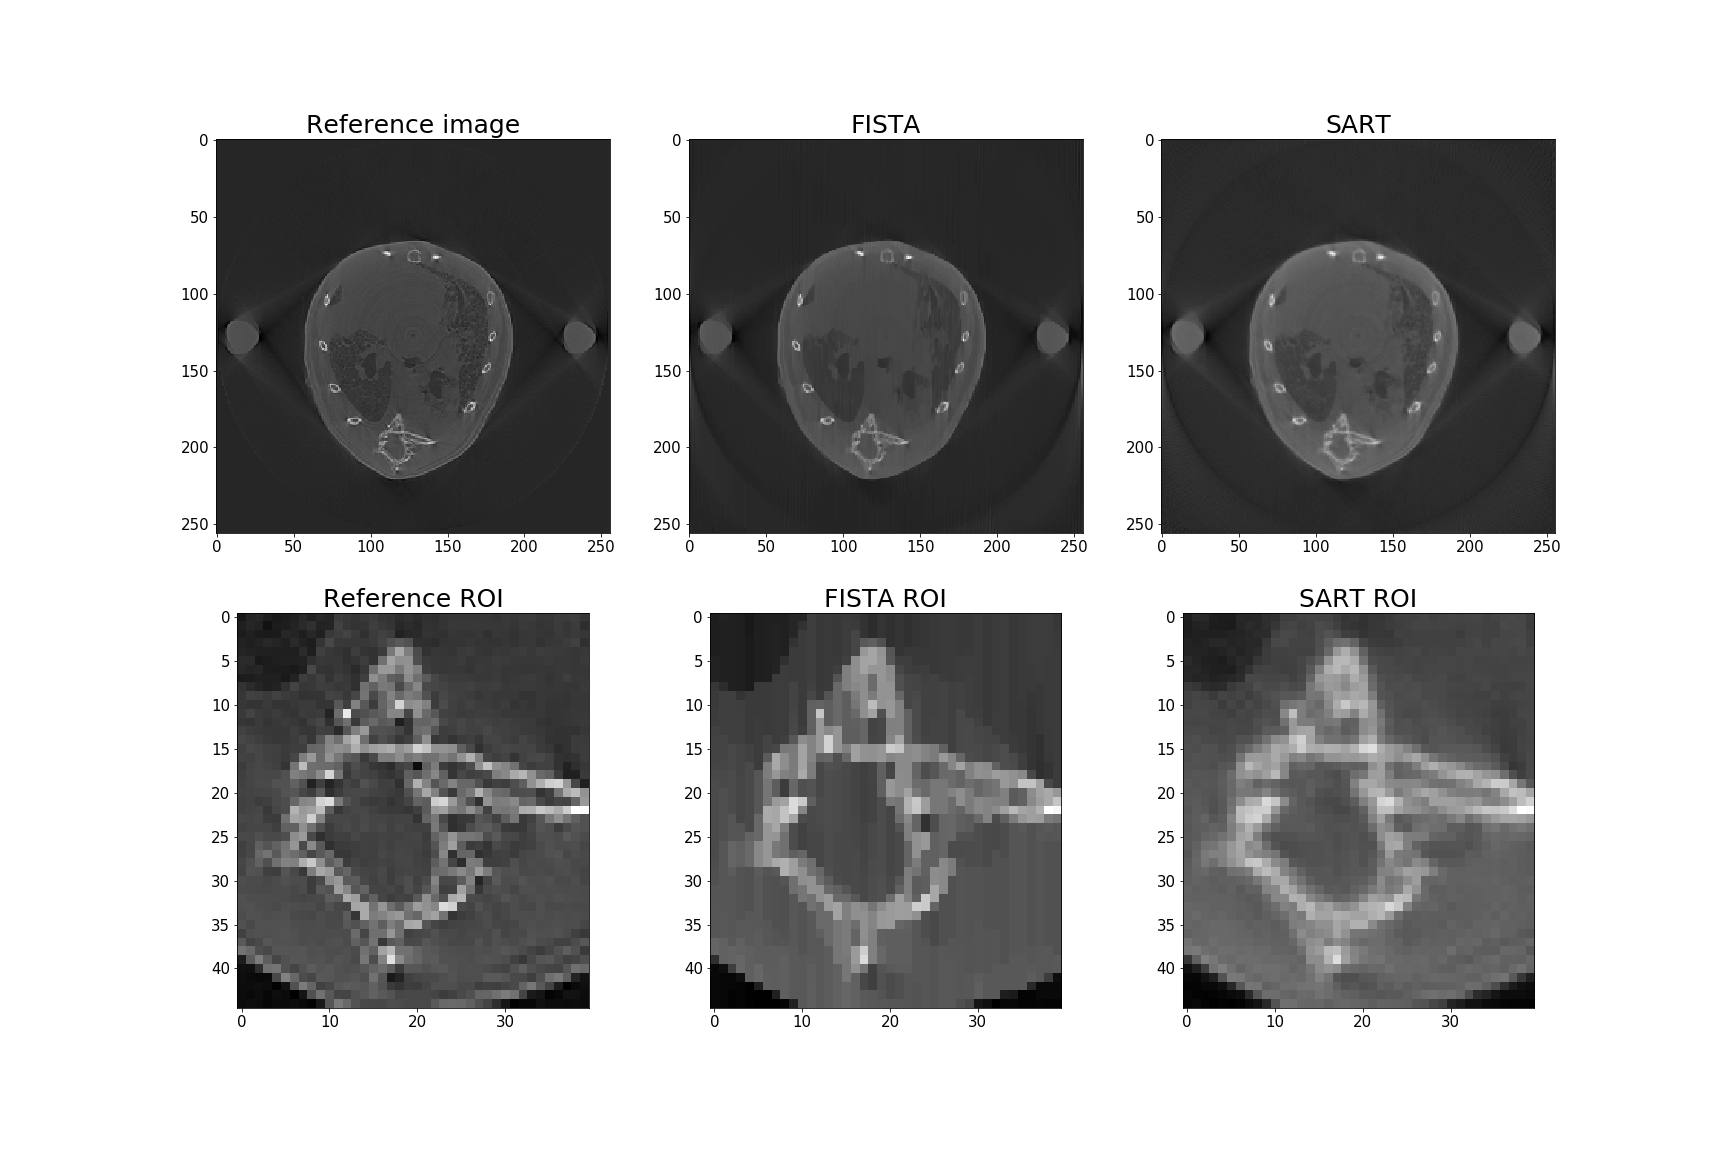
\includegraphics[height=0.35\paperheight]{../results/comparison270.png}
	\caption{Reconstructed image using FISTA and SART from the 270 views.}
	\label{fig:comparison270}
\end{figure}

% FISTA and SART side by side: 90
\begin{figure}[H]
	\centering
	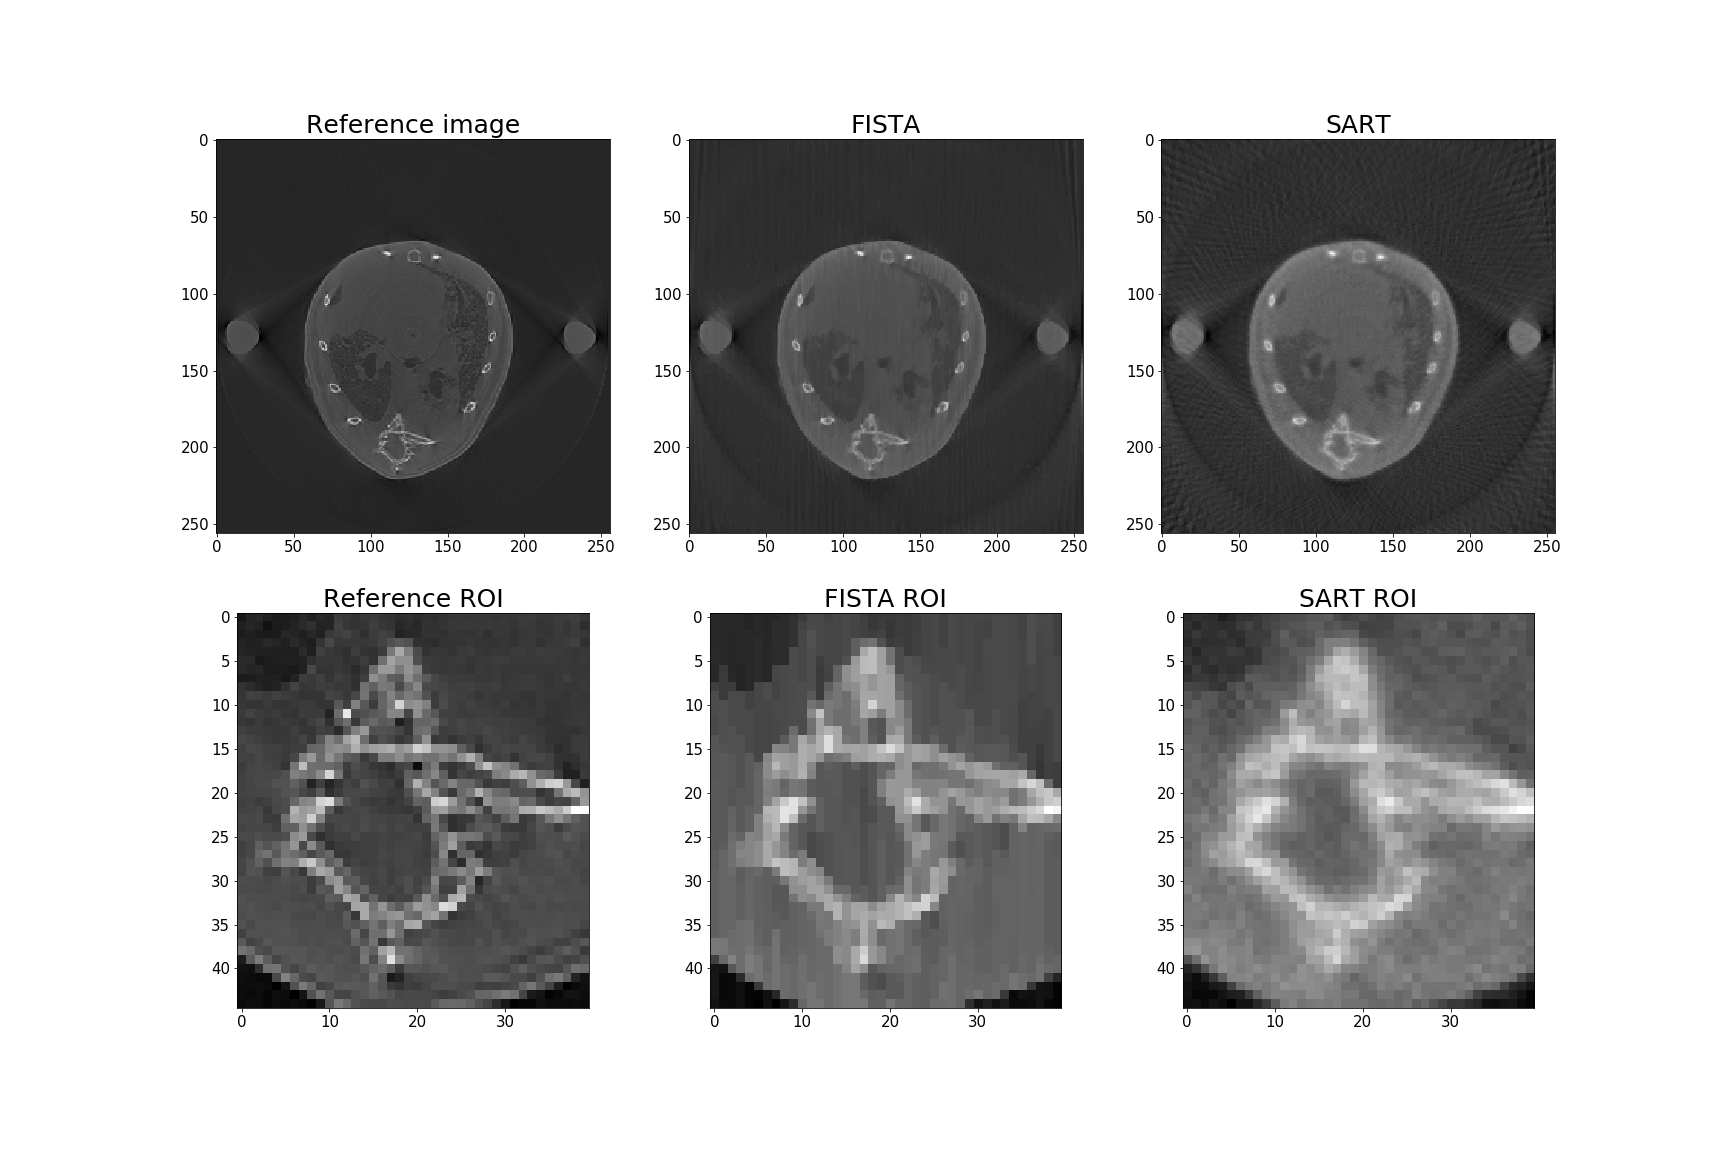
\includegraphics[height=0.35\paperheight]{../results/comparison90.png}
	\caption{Reconstructed image using FISTA and SART from the 90 views.}
	\label{fig:comparison90}
\end{figure}

\section{Discussion and Conclusions}
\noin In general, FISTA outperforms SART at reconstructing the image. By comparing reconstructions on the three different sinograms, we see that the SSIM and MSE is substantially more stable with FISTA (Tables~\ref{tab:ssim},~\ref{tab:mse}). Therefore, FISTA creates more robust reconstructions with less data. Although the global SSIM with the full sinogram is slightly higher for SART, this is because FISTA creates a sharper halo effect around the actual image (Figure~\ref{fig:comparisonfull}) likely due to the total variation regularization. Indeed, the SSIM over the ROI is better with FISTA than with SART and we can see that the colors and shading more closely resemble the reference image. The FISTA reconstruction also has sharper edges compared to the SART reconstruction. This is especially apparently as fewer views are used (Figure~\ref{fig:comparison270}). Finally, FISTA is much more tolerant to noise. In the 90 view reconstruction, the SART reconstruction contains wavy patterns whereas the FISTA reconstruction does not contain any noise artifacts (Figure~\ref{fig:comparison90}). As a result, the FISTA reconstruction over the ROI does a much better job preserving the complex structures. In addition, the SART reconstruction appears to have a much noisier, non-uniform background in the ROI.

\vspace{0.2in}

\noin To summarize, we conclude that FISTA creates more robust reconstructions with less data, creates sharper edges, and is more tolerant to noise than stationary iterative methods such as SART.

\section{Author Contributions}
\noin All authors contributed equally to this project. KD generated the forward operators and sinograms, chose image quality metrics, and wrote the Introduction and Problem Formuation. RF implemented SART, wrote the final code, and wrote the Resuts and Discussion sections. SZ wrote the pesudocode of the FISTA algorithm, developed prototype FISTA code, and wrote the Methods section.

\section{Code Availability}
\noin All code used for this project, with instructions for use, is available at \url{https://github.com/rfriedman22/ese5932_final_project/}.

\newpage
% Full image reconstructions
\setcounter{figure}{0}
\renewcommand{\thefigure}{S\arabic{figure}}
\begin{figure}[h]
	\centering
	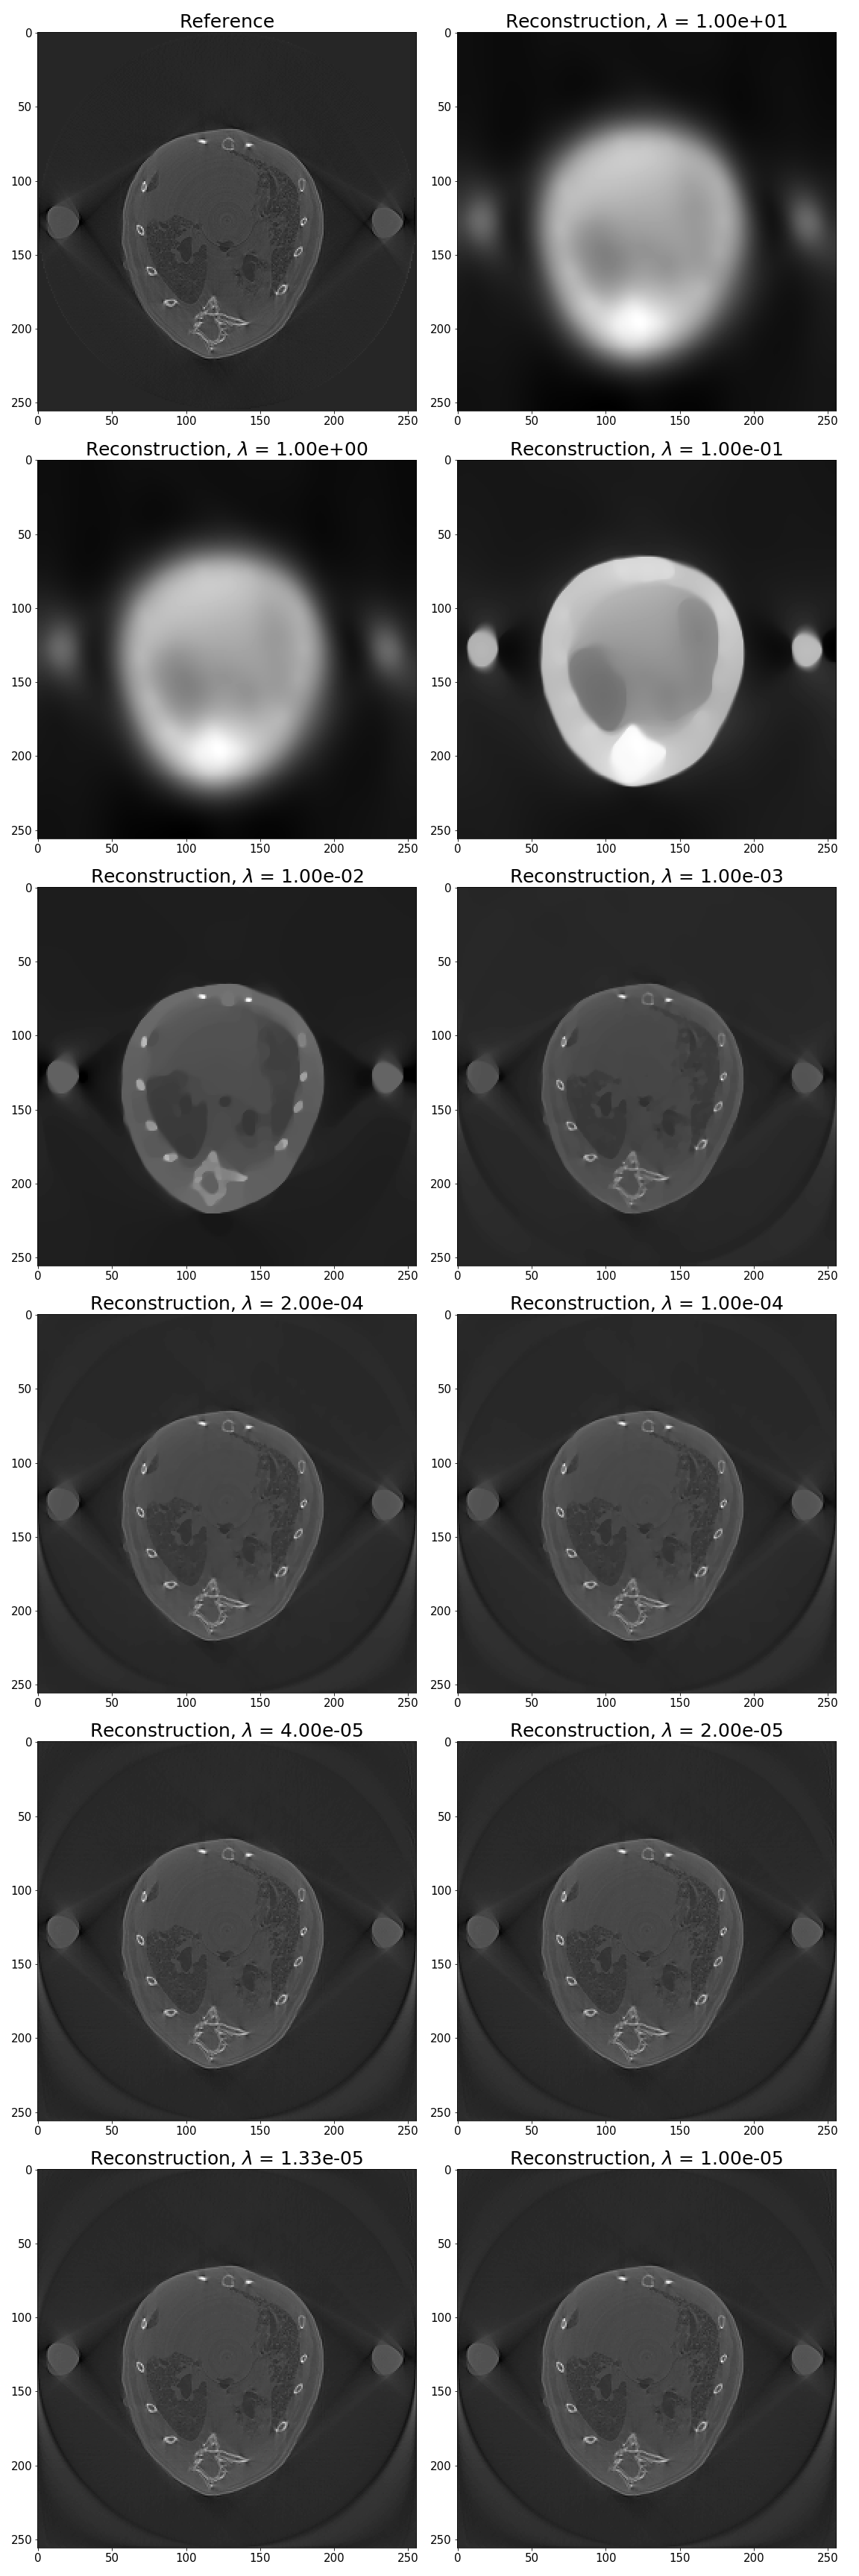
\includegraphics[height=0.8\paperheight]{../results/fistaFullImages.png}
	\caption{FISTA reconstruction from full sinogram with different values of $\lambda$.}
	\label{fig:fullReconstructions}
\end{figure}

\end{document}
